\section{Architecture \& Approach}
% OR: \section{Model}
\label{sec:architecture}
\subsection{Exploratory Data Analysis}
In this section we will go over the dataset chosen for this task, the preprocessing pipeline implemented as well as the a-priori insights we can extract regarding its contents.

\subsubsection{Dataset}
The dataset used in this analysis consists of speeches and statements gathered from the official website of the Office of the Greek Prime Minister in the time period between 2012 and 2024. It was fetched and assembled by a custom-built web page scraper, yielding approximately $2030$ distinct publications. 

The dataset is primarily in Greek, with a minority of English or French phrases/words. These publications are official transcripts and/or summaries of speeches and statements given by the active prime minister at the period. No other filtering was applied in the initial construction of the dataset other than the aforementioned time frame. While the speeches and the statements were loaded independently, a merged version of the data will be used in all of the tasks presented as they have an identical format, as shown in Table \ref{tab:dataset}.

\begin{table}[H]
\centering
\begin{tabular}{c|c|l}
\toprule
\textbf{Field} & \textbf{Type} & \multicolumn{1}{c}{\textbf{Description}} \\
\midrule
date   & str & Publication Date \\
id     & int & Publication ID \\
url    & str & Publication URL \\
title  & str & Publication Title \\
text   & str & Publication Content \\
\bottomrule
\end{tabular}
\caption{Dataset Attributes}
\label{tab:dataset}
\end{table}

\subsubsection{Data Preprocessing}
Our dataset consists of long texts in Greek, with a lot of repetitive language and - due to its context - legalese. OCTIS provides classes for easily preprocessing and storing the dataset, which may then be used as input in any of its algorithms for training and evaluation. One drawback of OCTIS' provided preprocessing is that it is black-box - it uses spaCy \citep{spacy:17} to modify the data and construct the expected dataset class. While spaCy provides support for processing Greek corpora, its lemmatization pipeline was unable to reduce most of the words to their root forms sufficiently. This was especially apparent in less mainstream words, which are quite common in official speeches and statements, as well as verbs. 

In order to overcome this issue we built a custom and OCTIS-compatible preprocessor based on Stanford's Stanza (\cite{Stanza:20}). Stanza supports the usage of external, custom-made models for the processing steps. While Greek is natively supported, we opted for a more specialized approach on lemmatization for the Greek language. As presented by \cite{Prokopidis;Piperidis:20} in A Neural NLP toolkit for Greek - their hybrid lexicon and part-of-speech based lemmatizer will be used so as to achieve more accurate conversions to root forms and therefore avoid the repetition of lexical cognates when generating topics. The difference between the two pipelines was not trivial and almost eliminated the issue of monolectic topics. With our pipeline prepared, there is a series of additional steps to be performed so as to build our training-ready dataset. 


Stopword removal will be applied using the union of spaCy's Greek el\_core\_news\_sm and English en\_core\_news\_sm. In fact, stopwords will be lemmatized and will be removed from the post-lemmatized text for higher coverage as Greek is quite a versatile language and these lists were not exhaustive. Removal of numbers and punctuation marks was also applied so as to have a more relevant vocabulary and ensure that words are not entangled between punctuation marks.

Word weighting with TF-IDF was used in order to maximize the relevance of the words present in our vocabulary in order to assist with the generation of topics. Specifically, all words present in more than $20\%$ or less than $1\%$ of the texts were omitted from the vocabulary. Additionally, a text had to consist of at least 20 words in order to be counted in as a data point. Finally, the minimum word length was set to 4, immediately excluding a plethora of context-lacking phrases. 

While the OCTIS models require preprocessing in order to produce acceptable result, unlike BERTopic which according to its documentation performs better when the input data is unprocessed and performs data processing later in its pipeline.

\subsubsection{Understanding The Data}
Instead of tackling the task blind, it is generally a good idea to extract some statistics prior to the analysis. This helps in spotting possible biases, imbalances or errors in the dataset.

\begin{figure}[H]
\centering
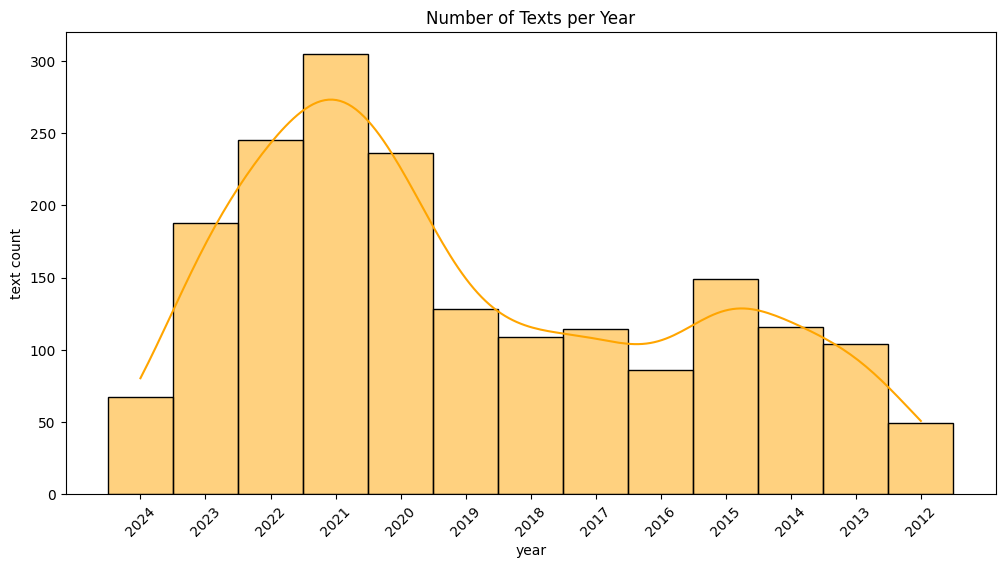
\includegraphics[width=0.8\columnwidth]{figs/eda_texts.png}
\caption[]{Count of data samples per year}
\label{fig:EDA_texts}
\end{figure}

As seen in Figure \ref{fig:EDA_texts}, our data is imbalanced in the sense that there has been a lot of publication activity from the Office of the Greek Prime Minister in the post-COVID era, meaning we might see an increased amount of recent topics compared to the mid-2010's. 

\begin{table}[H]
\centering
\caption{Selected Common Words by Year}
\label{tab:commonwords}
\begin{tabular}{@{}p{1cm}p{5cm}p{4cm}@{}} % Adjust the column width and alignment if necessary
\toprule
\textbf{Year} & \textbf{Common Words} & \textbf{Topic Description} \\
\midrule
2022 & \textgreek{ενεργειακός, ψηφιακός, τουρισμός, πηγή, πόλεμος} & Energy, Digital, Tourism, War \\
2021 & \textgreek{εμβολιασμός, ψηφιακός, εμβολιάζω, υφυπουργός, γραμματέας} & Vaccines, Digital Campaigns \\
2018 & \textgreek{μνημόνιο, περιφέρεια, παραγωγικός, νησί} & Memorandum, County, Island \\
2013 & \textgreek{πλεόνασμα, κόμμα, ανταγωνιστικότητα, ανεργία} & Surplus, Competitiveness, Unemployment \\
\bottomrule
\end{tabular}
\begin{tablenotes}
  \small
  \item \textit{Complete table available at Appendix \ref{sec:appA} Table \ref{appA:words_per_year}}
\end{tablenotes}
\end{table}



As we see in Table \ref{tab:commonwords}, we can also take a quick look at the most common words that appear in our texts, per year, as a taste of what to expect when generating topics.

\subsection{OCTIS Models}

Optimizing and Comparing Topic Models Is Simple (OCTIS) (\cite{Terragni;Fersini;Galuzzi;Tropeano;Candelieri;21}) is a library that encapsulates the preprocessing, optimization, training, evaluation and comparison of topic models. It contains a plethora of topic model algorithm implementations and metrics and thus will be used throughout so as to provide a platform for our chosen methods in this analysis. In this sub-section we will briefly go over the OCTIS-provided algorithms we will use in our experiments.

\subsubsection{Latent Semantic Indexing} 
Latent Semantic Indexing (also known as Latent Semantic Analysis, \cite{Landauer;Thomas;Foltz;Peter;Laham;Darrell:98}) is one of the first approaches in topic modeling that attempts to overcome the issue of variability in language when trying to retrieve relevant topics. It is able to extract context and capture semantic similarities between different words.

The algorithm initially constructs a weighted document-term matrix which stores the importance of each word based both on term frequency and inverse document frequency (tf-idf). This high-dimensional sparse matrix is then decomposed into three intermediate matrices using Singular Value Decomposition (SVD). These matrices are the term-concept vector matrix $W$, the singular value matrix $S$ and the concept-document vector matrix $P$. By picking the most significant singular values (columns) from $S$, the original matrix is essentially truncated and thus its dimensionality is reduced while keeping the maximum possible context. 

\subsubsection{Latent Dirichlet Allocation}
Latent Dirichlet Allocation (LDA) (\cite{Blei;Ng;Jordan:03}) is a generative probabilistic model designed for the analysis and decomposition of collections of discrete data sets into a predetermined number of topics. It is predicated on the construction of a Bayesian model where documents are conceptualized as random mixtures over latent topics and each topic is characterized by a specific distribution over words. Documents are generated by sampling words from these topic-specific distributions.

It fundamentally operates using a fixed K-dimension Dirichlet distribution. As seen in Figure \ref{fig:LDA_Plate}, the parameters include $\alpha$ and $\beta$, which are hyperparameters that set the prior distributions over document-topic mixtures and topic-word mixtures respectively. Additionally, $\theta$ represents the distribution of topics in a specific document. Finally, $z$ assigns topics to individual words and $w$ denotes the distribution of words for each topic, capturing the semantic essence. This assignment over the $N$ words is repeated for all the documents $D$.

\begin{figure}[H]
\centering
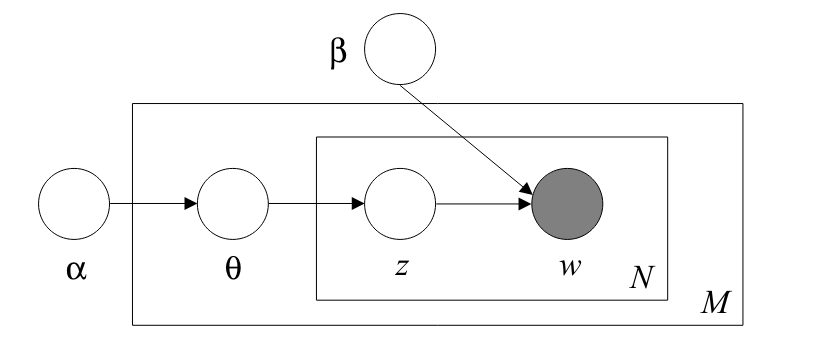
\includegraphics[width=0.5\columnwidth]{figs/lda_plate.png}
\caption[Latent Dirichlet Allocation Plate]{Plate representation of LDA
(adapted from \cite{Blei;Ng;Jordan:03})}
\label{fig:LDA_Plate}
\end{figure}

\subsubsection{Hierarchical Dirichlet Process} 
%https://www.cs.cmu.edu/~epxing/Class/10708-14/scribe_notes/scribe_note_lecture20.pdf
%https://mlg.eng.cam.ac.uk/zoubin/tut06/ywt.pdf
%https://people.eecs.berkeley.edu/~jordan/papers/hdp.pdf
%https://www.gatsby.ucl.ac.uk/~ywteh/research/npbayes/dp.pdf

Hierarchical Dirichlet Process (HDP) \citep{Teh;Jordan;Beal;Blei:06} is a topic modeling technique that extends the capabilities of LDA by allowing for an infinite number of topics across documents. While LDA requires pre-specifying dimensionality of the Dirichlet distribution (number of topics), HDP overcomes this limitation by leveraging the Dirichlet Process (DP) to model a potentially infinite number of topics, thereby providing a more flexible modeling approach. DP is an extra level added to the model.

\subsubsection{Product of Experts Latent Dirichlet Allocation}
%https://arxiv.org/pdf/1703.01488.pdf

Product of Experts Latent Dirichlet Allocation (ProdLDA) \citep{Srivastava;Sutton:17}, is a topic model that enhances the conventional LDA by modifying its underlying generative process. Unlike LDA, which represents documents as mixtures of topics where each word's generation is attributed to a single topic, ProdLDA redefines this structure by modeling the generation of words in a document as a Product of Experts \citep{hinton1999products}.

This simple yet important distinction allows ProdLDA to overcome a limitation of LDA where its generative process tends to yield less specific, and at times, less interpretable topics because the likelihood of word generation is averaged over the topics. 


\subsubsection{Honorable Mentions}
% %(https://papers.nips.cc/paper_files/paper/2000/hash/f9d1152547c0bde01830b7e8bd60024c-Abstract.html)

Non-negative Matrix Factorization (NMF) is a machine learning algorithm aimed at reducing the dimensionality of non-negative data by breaking it down into two matrices revealing underlying patterns, similar to LSI. While not natively a topic model, it is popular thanks to its ability to reduce dimensionality and produce coherent topics.

\subsection{BERTopic}
\label{sec:bertopic}

The previously mentioned algorithms rely on bag-of-word representations, which ignore the semantic relationships between words. Word embeddings and the emergence of Transformer-based models, such as Bidirectional Encoder Representations from Transformers (BERT) \citep{devlin2019bert} allow texts to be represented in such a way that similar texts are put together in the vector space. Then, as proposed by \citeauthor{sia-etal-2020-tired} \citeyearpar{sia-etal-2020-tired}, those embeddings can be clustered with each cluster representing a different topic.

BERTopic \citep{grootendorst2022bertopic} builds on this and combines clustering with a novelty class-based TF-IDF (c-TF-IDF) to create coherent topics from the created clusters. 

The steps of a BERTopic process, as seen in Figure \ref{fig:bertopic_architecture}, include creating embeddings of the documents, reducing the dimensions of those embeddings and then performing clustering. After that c-TF-IDF weighs the words present in each cluster to create topic representations.

\begin{figure}[H]
\centering
\includesvg{figs/bertopic.svg}
\caption[https://maartengr.github.io/BERTopic/algorithm/algorithm.html]{BERTopic Architecture (figure from Grootendorst Maarten)\footnotemark}}
\label{fig:bertopic_architecture}
\end{figure}
\footnotetext{https://maartengr.github.io/BERTopic/algorithm/algorithm.html}

BERTopic's other advantage lies in its modularity where each step algorithm of each step can be replaced with a different one.

\subsubsection{Sentence Transformers}
Similar to how traditional word embedding techniques create numerical vectors to make word representations, sentence transformers, as the name suggests, are able to generate embeddings for a large collections of tokens, creating vector representations for whole documents, sentences or paragraphs.

BERTopic for this step uses the Sentence-BERT (SBERT) framework \citep{reimers2019sentencebert} which consists of pre-trained Transformer-based language models. The SBERT framework provides many pre-trained models but any model can be used for creating text representations, such as models provided by Spacy, Gensim and Scikit-Learn Embeddings,

\subsubsection{Uniform Manifold Approximation and Projection for Dimension Reduction (UMAP)}
Sentence embeddings created by SBERT exist in a high dimensional space and, as found by \citeauthor{steinbachChallengesClusteringHigh2004} and \citeauthor{10.1007/3-540-49257-7_15}, traditional clustering techniques don't work well in high dimensions. The solution to that is reducing the dimensions. 

Techniques such as Principal Component Analysis (PCA) and t-Distributed Stochastic Neighbor Embedding (t-SNE) are widely used dimensionality reduction but BERTopic uses UMAP \citep{mcinnes2020umap}, which has shown to better preserve local features when reducing to as low as 2 dimensions.
\subsubsection{HDBSCAN}
After the document embeddings have reduced in dimensions, the clustering is performed with a hierarchical variation of Density-Based Spatial Clustering of Applications with Noise (DBSCAN).


DBSCAN \citep{10.5555/3001460.3001507} is a clustering algorithm that identifies dense regions of points that exist within a certain distance from each other and adding them to the same cluster. More specifically, it works with two parameters: \textgreek{ε}, which specifies the radius of the circle around each data point and minimum points, which specifies the least amount of points needed to form a cluster. Points with enough neighbors are core points of a cluster, whereas points far from any neighborhood are classified as noise.

Hierarchical DBSCAN (HDBSCAN) \citep{McInnes2017} performs DBSCAN with varying epsilon values, trying to find the one that gives the best stability. In this way, clusters of varying densities are created.

\subsubsection{c-TF-IDF}
Each cluster created by HDBSCAN represents a single topic. Depending on our corpus, each cluster may include hundreds or more words and we need to find a meaningful way to represent each cluster. 

\begin{equation}\label{c-tf-idf}
W_{t,c} = tf_{t,c} \cdot \log(1 + \frac{A}{tf_{t}})
\end{equation}

As seen in Equation (\ref{c-tf-idf}) the frequency of a term $t$ is calculated for an entire cluster $c$. Then, instead of the inverse document frequency, we calculate the inverse \textit{class} frequency, measuring how much information a term provides in an entire cluster.

\subsubsection{Topic Representation Fine-Tuning}
BERTopic's final component focuses on how the created topics can be represented. Although the default topic representations created with c-TF-IDF are representative of the general theme of each topic they can sometimes be misleading as, due to c-TF-IDF's nature, rely on word frequency. As a result the most semantically relevant words may be ignored and many topics end up with a similar representation. While all the previous components played a crucial role in how the topic clusters are created, representation models play a more qualitative role. These models can vary from Part of Speech matchers, Maximal Marginal Relevance Calculation, keyword extractors such as KeyBERTInspired and even Large Language Models such as Generative Pretrained Transformers. Any combination of these different models can be combined in a chain model, where multiple representation models are used in succession with the output of one being the input of the next one.

KeyBERTInspired is an adaptation of KeyBERT \citep{grootendorst2020keybert}. KeyBERT creates embeddings of both each document and each word in the document. Afterwards it calculates the cosine similarities between the word and document embeddings to find the words that are most similar to the document. Those words are considered to be the most representative.

Maximal Marginal Relevance (MMR) \citep{10.1145/290941.291025} on the other hand works by trying to calculate both the relevance of a word within a document, and its diversity among other words in the document. This helps avoid having very similar words as the topic representation.
